\documentclass[border=1cm]{standalone}

\usepackage{tikz}

\begin{document}
    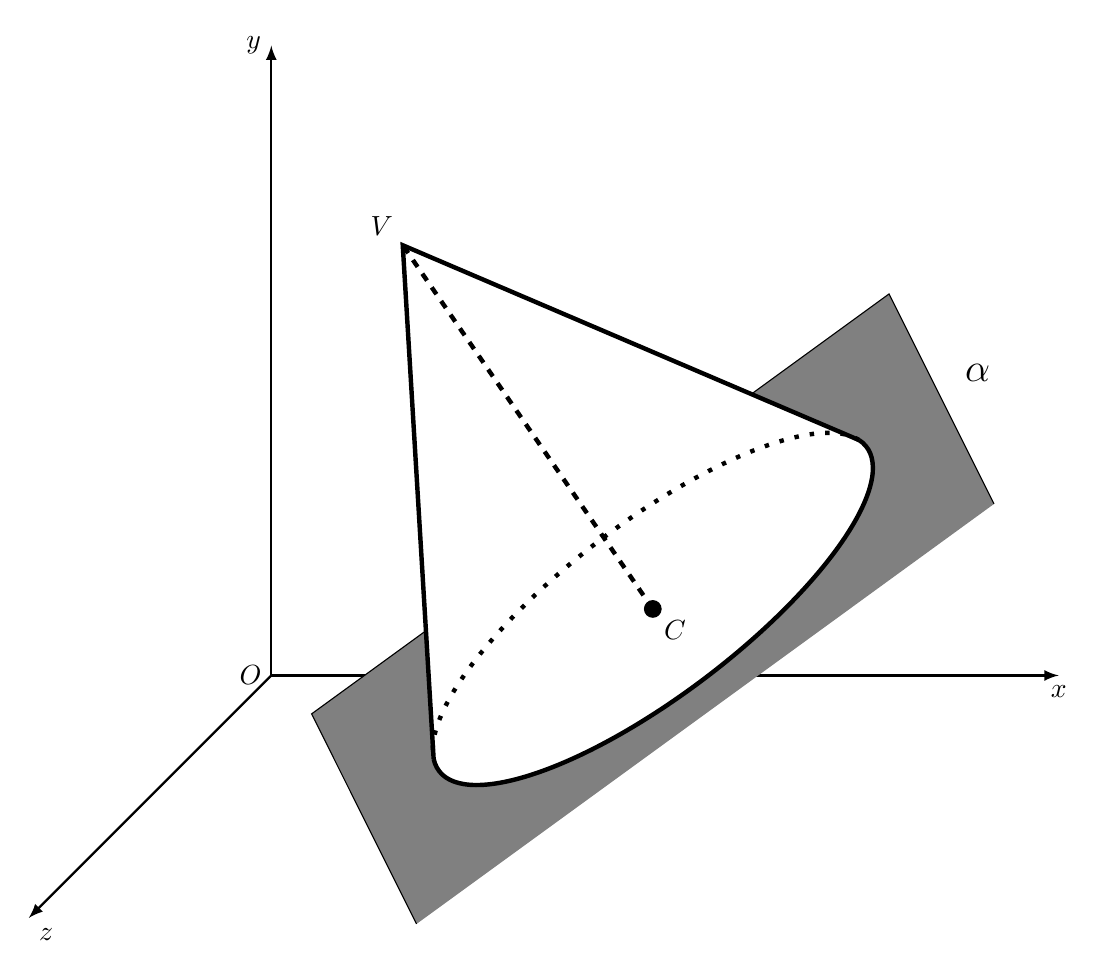
\begin{tikzpicture}
        \draw[->,>=latex,thick](0,0)--(10,0)node[below]{$x$};
        \draw[->,>=latex,thick](0,0)--(0,8)node[left]{$y$};
        \draw[->,>=latex,thick](0,0)--(0,0,8)node[below right]{$z$};
        \node at (0,0) [left]{$O$};
        \begin{scope}[shift={(6,2,3)}, rotate around y=-60, rotate around x=-60]
            \draw[fill=gray] (45:{4*sqrt(2)})--(135:{4*sqrt(2)})--(225:{4*sqrt(2)})--(315:{4*sqrt(2)});
            \filldraw[white] (0,0) circle [radius=3];
            \draw[ultra thick] (-95:3) arc [start angle=-95, end angle=100, radius=3];
            \draw[ultra thick,fill=white] (100:3)--(0,0,6)--(-95:3);
            \draw[ultra thick, loosely dotted] (100:3) arc [start angle=100, end angle=265, radius=3];
            \draw[ultra thick, dashed] (0,0)node[below right]{$C$}--(0,0,6);
            \draw[fill] (0,0) circle [radius=3pt];
            \node at (0,0,6) [above left]{$V$};
            \Large
            \node at (90:4.5) {$\alpha$};
        \end{scope}
    \end{tikzpicture}
\end{document}